\documentclass[11pt]{article}
%you can look for fun LaTeX packages to use hereasdf

\usepackage{amsmath}
\usepackage{amssymb}
\usepackage{fancyhdr}
\usepackage{amsthm}

\usepackage{graphicx}
\usepackage{dcolumn}
\usepackage{bm}

%fun commands for fun sets
%make sure to use these in math mode
\newcommand{\Z}{\mathbb{Z}}
\newcommand{\R}{\mathbb{R}}
\newcommand{\N}{\mathbb{N}}
\newcommand{\C}{\mathbb{C}}
\newcommand{\m}{\mathcal{M}}
\newcommand{\Tt}{\mathcal{T}}
\newcommand{\pa}{\partial}
\newcommand{\dD}{\mathcal{D}}
\newcommand{\E}{\mathbb{E}}



\oddsidemargin0cm
\topmargin-2cm    
\textwidth16.5cm   
\textheight23.5cm  

\newcommand{\question}[2] {\vspace{.25in} \hrule\vspace{0.5em}
\noindent{\bf #1: #2} \vspace{0.5em}
\hrule \vspace{.10in}}
\renewcommand{\part}[1] {\vspace{.10in} {\bf (#1)}}

\newcommand{\myname}{Alex Havrilla}
\newcommand{\myandrew}{alumhavr}
\newcommand{\myhwnum}{Hw 1}

\newtheorem{theorem}{Theorem}
\newtheorem{prop}{Prop}
\theoremstyle{remark}
\newtheorem{lemma}{Lemma}
\newtheorem{remark}{Remark}
\newtheorem{defi}{Def}
\newtheorem{apps}{Application}
\newtheorem{quest}{Question}
\newtheorem{ans}{Answer}
\newtheorem{interest}{Interesting}
\newtheorem{theme}{Theme}
\newtheorem{back}{Background}
\newtheorem{idea}{Idea}
\newtheorem{example}{Example}
\newtheorem{reminder}{Reminder}

\setlength{\parindent}{0pt}
\setlength{\parskip}{5pt plus 1pt}
 
\pagestyle{fancyplain}
\lhead{\fancyplain{}{\textbf{HW\myhwnum}}}      % Note the different brackets!
\rhead{\fancyplain{}{\myname\\ \myandrew}}
\chead{\fancyplain{}{\mycourse}}

\linespread{1.3}

\title{Feb Log}

\begin{document}

\maketitle

\section{1/31}

\subsection{Chess}

\begin{remark}
	A blunder free game with weak positional moves:
	\begin{verbatim}
		https://www.chess.com/analysis/game/live/6409740211?tab=analysis
	\end{verbatim}
\end{remark}

\begin{remark}
	A complicated blunder filled game:
	\begin{verbatim}
		https://www.chess.com/a/CbAJ8Wm4XAX8
	\end{verbatim}	

	To Analyze:
\end{remark}

\subsection{Complex Analysis}

\section{2/1}

\subsection{Chess}

\begin{remark}
	Talk about a clean game:
	\begin{verbatim}
		https://www.chess.com/a/Gzp6PJxWXAX8
	\end{verbatim}
\end{remark}

\begin{remark}
	My first brilliant move!:
	\begin{verbatim}
		https://www.chess.com/a/2BfrDrz2JXAX8
	\end{verbatim}
\end{remark}



\subsection{Technical Animation}

\begin{interest}
	TA Arjun is interested in PDEs and numerical simulation.
\end{interest}

\begin{remark}
	Course Website:
	\begin{verbatim}
		http://graphics.cs.cmu.edu/nsp/course/15464-s21/www/
	\end{verbatim}

	\textit{Computer Animation: Algorithms and Techniques} is the course textbook. In drive.
\end{remark}

\begin{quest}
	Does greater physical simulation accuarcy lead to a less palatable viewing experience? 
\end{quest}

\begin{ans}
	Not sure but often directors will personify animations and we have different parameters to give differenter personfications. For example "angry storm".
\end{ans}

\begin{ans}
	It seems exaggerated motion is often more digestestible(think actors for example). Often used actors in motion capture
\end{ans}

\begin{interest}
	Rig Net: automatically rigging meshes. Note: rigging is process of jointing meshes, providing structure/skeleton.
\end{interest}

\begin{remark}
	Beginning of rigging: find medial axis of geometry and impose some structure.
\end{remark}

\subsection{On Lp Brunn-Minkowski Type Inequalities}

\textbf{Tag}: BrunnMinkowski

\begin{remark}
	V is $1/n$ concave measure w.r.t Minkowsi sum. Need normalizing $1/n$ powers 
\end{remark}

\begin{prop}
	\begin{align*}
		h_{K+L}(u) = h_K(u) + h_L(u)
	\end{align*}
\end{prop}

\begin{remark}
	\textbf{Brascamp-Lieb}

	$\alpha \geq -1/n, t\in [0,1]$. With $f,g,h : \mathbb{R}^n \to \mathbb{R}_+$ satisfy

$h((1-t)x + ty) \geq [(1-t)f(x)^{\alpha} + tg(y)^{\alpha}]^{1/\alpha}$ then

$\int_{R^n} h(x)dx \geq [(1-t)(\int_{R^n}f(x)dx)^{\alpha/1+n\alpha}+t(\int_{R^n}g(x)dx)^{\alpha/1+n\alpha}]^{1+n\alpha/\alpha}$

Prekopa lindler is $\alpha = 0$
\end{remark}

\begin{prop}
	\begin{align*}
		(1-t)X_s1_A \oplus_s t X_s 1_B = 1_{(1-t)A + tB}
	\end{align*}
\end{prop}

\begin{remark}
	Changing operator: minkwoski sum, to $l_p$ variants. 
\end{remark}

\begin{remark}
	Also some kind of interplay beteween functional inequalities and volume inequalities. Between supremal convolutions and Lp minkwoski sums.
\end{remark}

\subsection{PDEs and Data Analysis}

\textbf{TAG:} OptimalTransport

\begin{theme}
	The more assumptions you make on a measure the better approximation you can achieve
\end{theme}

\begin{interest}
	Shimaa is interested in stochastic BDEs. Wes interested in foundations of machine learning.
\end{interest}

\begin{theme}
	Look at a measure as some kind of energy landscape and the transport map as the process of rearranging mass.
\end{theme}

\begin{remark}
	Often transportation cost is $|x-y|^p$. 
\end{remark}

\begin{remark}
	Optimal transport minimizes transportation cost.
\end{remark}

\begin{theme}
	Goal is to find weaker problem which provides good solution to wider class of subproblems.
\end{theme}


\section{2/2}

\subsection{Goals}

\begin{enumerate}
	\item Chess: 1300 in blitz
	\item Research: 3 hours worked, some progress, email tkocz
	\item Thesis: 5 pages
	\item Homework: Animation
	\item Get glenn to agree to a time
\end{enumerate}

\subsection{DRL}

\textbf{TAG:} DRL

\begin{quest}
	what is computational design?
\end{quest}

\begin{remark}
	Course link: 
	\begin{verbatim}
		https://cmudeeprl.github.io/403_website/
	\end{verbatim}
\end{remark}

\begin{remark}
	Katerina F.
	\begin{verbatim}
		"My genes have strong priors from the world"
	\end{verbatim}
\end{remark}

\begin{remark}
	Inconsistent rewards lead to addiction.
\end{remark}

\begin{remark}
	For a long time large emphasis on discovering new behaiors in DRL. Now thinking we need to develop behavior repetoire and associate with some stimuli.
\end{remark}

\begin{remark}
	Curiosity, a desire to see new things, very intrinsically powerful.
\end{remark}

\begin{remark}
	Conor Igoe: 
	\begin{verbatim}
		For a fixed known opponent, the evolution of chess is markovian from the perspective of the main player.
	\end{verbatim}

	In some cases(such as driving) we need multiple frames/time steps to even attempt to play. But this can also be redefined as markovian by letting states correspond to multiple time steps.
\end{remark}

\begin{remark}
	Model vs. non-model based. Can we learn via simulation or not.
\end{remark}

\begin{remark}
	Cannot use gradient based optimization often in DRL. We can if we have a model.
\end{remark}

\subsection{The Embodiment Hypothesis}

\begin{remark}
	Link:
	\begin{verbatim}
		https://cogdev.sitehost.iu.edu/labwork/6_lessons.pdf
	\end{verbatim}
\end{remark}

\begin{remark}
	The six lessons from child deveopment:
	\begin{enumerate}
		\item Be multimodal
	\end{enumerate}
\end{remark}


\subsection{Modeling Evolution}

\begin{remark}
	Selection or drift: tug of war between determinism and randomness.
\end{remark}

\subsection{Chess}

\begin{remark}
	For tactics, look for forcing moves.
\end{remark}

\begin{remark}
	Backrank pawns are massive!!! 
	\begin{verbatim}
		https://www.chess.com/puzzles/problem/1227605
	\end{verbatim}
\end{remark}



\section{2/3 and 2/4}

\subsection{Goals}

2/3

\begin{enumerate}
	\item Research 3 hours
	\item Thesis 5 pages
	\item 1300 blitz
\end{enumerate}

2/4

\begin{enumerate}
	\item Research 3 hours
	\item Thesis 5 pages
	\item 1300 blitz
\end{enumerate}

\subsection{Technical Animation}

\textbf{TAG:} TechnicalAnimation

\begin{remark}
	L-systems developed to describe plant structures and generation.
\end{remark}

\begin{remark}
	Tools for good animation: The Anmimators Survival Kit.
\end{remark}

\begin{remark}
	Idea behind rigging: for easy animating want ball control points you can manipulate for convenience.
\end{remark}

\begin{remark}
	Cloth simulation involves a mesh...
	Cloth intersection problems in Pixar's Coco:
	\begin{verbatim}
		https://www.researchgate.net/publication/326907399_Better_collisions_and_faster_cloth_for_Pixar's_Coco
	\end{verbatim}
\end{remark}

\begin{remark}
	Traditional animation: keyframing. 

	New variant: procedural animation. Often used for crowd animation.
\end{remark}

\begin{interest}
	Interesting site:
	\begin{verbatim}
	www.massivesoftware.com
	\end{verbatim}
\end{interest}

\begin{interest}
	Character controller using Motion VAEs interesting.
\end{interst}



\subsection{Complex Analysis}

\textbf{TAG:} ComplexAnalysis

\begin{remark}
	Cauchy riemann equations derived via simply differentiating f as a function of two varibles in real and comlex directions.
\end{remark}

\begin{quest}
	Cauchy riemann conditions are necessary. Are they sufficient?
\end{quest}

\begin{ans}
	Yes. 
	\begin{theorem}
		Let $f : \Omega \to \C$ with $f = u + iv$ and satisfying cauchy riemann. Then f is holomorphic.
	\end{theorem}
	\begin{proof}
		Fix $z_0 = x_0 + i y_0$.
		\begin{align*}
			u(x_0+h_1,y_0+h_2) = u(x_0,y_0) + u_xh_1 + u_y h_2 + o(h)
		\end{align*}

		and similarly for v. Then write $f(z_0 + h) - f(z_0)$ in terms of above and massage using cauchy riemann to get form $ah + o(h)$. 
	\end{proof}
\end{ans}

\begin{remark}
	Determinant of jacobian is really magnitude of norm of complex derivative squared.
\end{remark}

\begin{example}
	$f(x,y) = \sqrt{|x||y|}$ satisfies cauchy riemann but is  not holomorphic. 
\end{example}

\begin{theorem}
	Radius of convergence R of power series is
	\begin{align*}
		R = \frac{1}{limsup |a_n|^{1/n}}
	\end{align*}
\end{theorem}

\begin{proof}
	Idea is to compare to geometric series. Set R as desired. Then just compute(since we used limsup) and see that geometric series converges and or diverges in desired cases. This is also why we have problems on boundary. 
\end{proof}

\subsection{Chess}

\begin{remark}
	A beautiful positional/material tradeoff emerged:
	\begin{verbatim}
		https://www.chess.com/a/36gbqDERtXAX8
	\end{verbatim}

	After analysis apparently not that good?
\end{remark}

\begin{remark}
	The nastiest checkmate I've ever given:
	\begin{verbatim}
	https://www.chess.com/analysis/game/live/6441231672?tab=analysis
	\end{verbatim}
\end{remark}

\begin{remark}
	Sharp tactic game:
	\begin{verbatim}
	https://www.chess.com/analysis/game/live/6442135074?tab=analysis
	\end{verbatim}
\end{remark}

\begin{remark}
	Playing more interesting games:
	\begin{verbatim}
	https://www.chess.com/analysis/game/live/6443227668?tab=analysis
	\end{verbatim}
\end{remark}

\begin{remark}
	Really shouldn't have resulted in a pawn structure that lead to a passed pawn for opponent
	\begin{verbatim}
	https://www.chess.com/analysis/game/live/6443636791?tab=analysis
	\end{verbatim}
\end{remark}



\subsection{PDE and Data}

\textbf{TAG:} OptimalTransport

\begin{remark}
	Villani's Optimal Transport: New and Old
	\begin{verbatim}
		https://ljk.imag.fr/membres/Emmanuel.Maitre/lib/exe/fetch.php?media=b07.stflour.pdf
	\end{verbatim}
	Presented from a probabilistic perspective.
\end{remark}

\begin{remark}
	Via CoV, condition for transport map:
	\begin{align*}
		\rho(x) = \eta(T(x)) |det(DT(x))|
	\end{align*}
\end{remark}

\begin{prop}
	Change of variables formula justified via above:
	\begin{align*}
		\int_Y f(y) d\nu(y) = \int_X f(T(x))d\mu(x)
	\end{align*}
\end{prop}

\begin{quest}
	When does measure preserving map even exist between $\mu$ on X and $\nu$ on Y. 
\end{quest}

\begin{example}
	Consider to the above the non-example $\mu(x) = 1$, $\nu(y_1) = \nu(y_2) = 1/2$. 
\end{example}

\begin{remark}
	Transport plan is generalization of transport map that has the source and target measures as its marginals. If  we have a transport map then $(I \times T)_{\sharp}\mu$ is a transport plan. Effectively pushing measure onto graph of T(note I is identity). 
\end{remark}

\begin{quest}
	Why does $\mu \times \nu$ not always work? 
\end{quest}

\begin{ans}
	It does.
\end{ans}

\begin{remark}
	Optimal Transport cost in terms of plans is always well defined since a plan exists and infimum is always a min(this is the Kantorovich formulation, first one is monge formulation)
	\begin{align*}
		C(\pi) = \int_{X \times Y} c(x,y) d\pi(x,y) = \int_{X \times Y} c(x,y) d(I \times T)_{\sharp} \mu = \int_X c(x,T(x))d\mu(x)
	\end{align*}
\end{remark}

\begin{quest}
	In kantorovich, how do we know infimum is always min?
\end{quest}

\textbf{TAG:} VariationalCalculus

\begin{prop}
	Norms are lsc
\end{prop}

\begin{example}
	Picture of lsc function:
	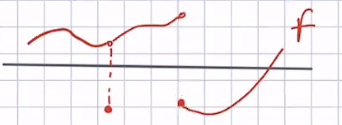
\includegraphics[width=250px]{C:/Users/Alex/Desktop/Notes/Spring 2021/pics/lsc.png}
\end{example}

\begin{prop}
	lsc functions achieve mins on compact sets
\end{prop}

\begin{proof}
	Let m inf. Let $x_n$ s.t. $f(x_n) \to m$. Sequential compactness gives us subsequence so that limit x stays in X. Thus $f(x)$ is minimizer since it must be smaller than all other valuations. 
\end{proof}

\begin{theorem}
	If X,Y compact and $c : X \times Y\to R$ then the kantorovich formulation has a solution
\end{theorem}

\begin{proof}
	\textbf{Proof using direct method of calculus of variations}

	$T_c : P(X\times Y) \to R$ is cts. w.r.t narrow convergence so $\int c \gamma = T_c(\gamma)$. Since $P(X \times Y)$ is tight and thus compact w.r.t narrow conv. Then if $\gamma_n \in \Pi(\mu,\nu)$ is a minimizing seq. then we have conv. subseq in product $P(X \times Y)$ for some $\gamma$. Need  $\gamma \in \Pi$. Doable by evauating marginals directly via  defintions above
\end{proof}

\begin{theme}
	We study measures by looking at test functions, which all for equality. Key idea is to look for notions which allow us to gai equality.
\end{theme}

\begin{prop}
	$\Pi(\mu,\nu)$ is convex.
\end{prop}

\subsection{DRL}

\textbf{TAG:} DRL

\begin{remark}
	Wolfer Ted Talk:
	\begin{verbatim}
		https://www.ted.com/talks/daniel_wolpert_the_real_reason_for_brains/transcript?language=en#t-1117820
	\end{verbatim}
\end{remark}

\begin{remark}
	Bayesian inference: data + prior knowledge informs action. Bayes rule: optimal rule for combining information.
\end{remark}

\begin{remark}
	We are sensory predictors detecting exterior sensory and subtracting off interior prediction.
\end{remark}

\begin{remark}
	Plan movements to minimize negative consequences of noise.
\end{remark}

\begin{remark}
	Q value is expected returns, not rewards. Must be learned from experience. They are predictive.
\end{remark}

\begin{remark}
	Intermediate reward shaping is hard because it can conflict and lead astray actions leading to final reward.
\end{remark}

\begin{quest}
	Why learn a model via supervised learning instead of hardcoding it in?
\end{quest}

\begin{ans}
	For some reason learning representation from data is very hard, even in supervised context. Representation is very important. Often times just don't generalize. This representation is more important in cases where we don't know how to hard code rules. This is a representation learning problem for the model, and representation is hard.
\end{ans}

\begin{quest}
	Do we use supervised learning to speed up the basic manipulation aquistition action?
\end{quest}

\begin{ans}
	In complex cases this is how the model must learn the world, because it cannot be "hard coded" in. 
\end{ans}

\begin{quest}
	Need more example of using supervised learning to learn dynamics model. Clearly not necessary in some cases.
\end{quest}

\begin{remark}
	Model free is no model, when is there is one it can be learned via supervised learning.
\end{remark}

\begin{quest}
	Why do we need supervised learning to learn dynamics in chess? Maybe it's just to predict the opponents move. 
\end{quest}

\begin{ans}
	Actually no it depends on if we include the opponent in the state or not but modula that its not really required if we have a "logical description" of the board. Sometimes neural network paramterizations of dynamics are nice though because they are less computationally expensive(than a newtonian description for example) and are differentiable(which is often useful).
\end{ans}

\begin{example}
	An example of both is controlling nuclear fusion power plant: there are great physics simulators that are quite accurate at predicting the next state, but they take on the order of 8 hours to solve a single second worth of real world dynamic. This is because the simulator is solving a very complex system of PDEs. In contrast, if we distill the dynamics into a neural network, it is much faster to simulate, and opens the door for novel planning and control techniques (at the cost of model bias)
\end{example}

\begin{theme}
	Theory and muscle learning are two ends of an extreme. Theory is exteremely generalizable but not particularly precise. Muscle learning is very precise but not particularly generalizable. This naturally occurs because the world is complex and more precision requires more information. How do we optimize between generalization and precision? This is the overfit problem
\end{theme}

\subsection{Chess}


\begin{remark}
	Insane game with no pawn captures:
	\begin{verbatim}
		https://www.chess.com/analysis/game/live/6448761849?tab=analysis
	\end{verbatim}

	The whole game I slowly let myself get backed into a corner
\end{remark}

\begin{remark}
	Try to use pawns to restrict play more
\end{remark}

\begin{remark}
	Need to exploit weakness:
	\begin{verbatim}
		https://www.chess.com/analysis/game/live/6449777852?tab=analysis
	\end{verbatim}

	When opponent exposes weakness(structural) need to identify and exploit.
\end{remark}

\begin{remark}
	What's better than e6 in modern?
	It was good in this game:
	\begin{verbatim}
		https://www.chess.com/analysis/game/live/6451734999?tab=analysis
	\end{verbatim}
	It allowed me to challenge center and break open for rook without weakening pawns too much
\end{remark}

\begin{remark}
	Complete dominance:
	\begin{verbatim}
		https://www.chess.com/analysis/game/live/6453705068?tab=analysis
	\end{verbatim}
	
\end{remark}


\subsection{Modeling Evolution}

\textbf{TAG:} ModelingEvolution

\begin{example}
	Reframing change in terms of dependent variable:
	
	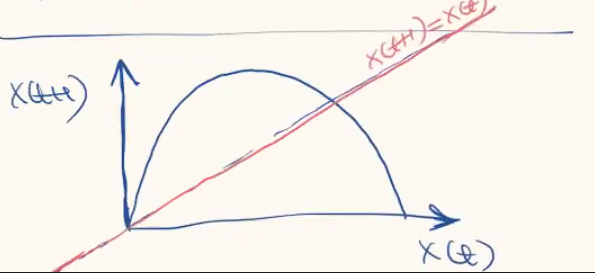
\includegraphics[width=250px]{C:/Users/Alex/Desktop/Notes/Spring 2021/pics/growth.png}
\end{example}

\section{2/5}

\subsection{Goals}

\begin{enumerate}
	\item 1350 chess
	\item Research 3 hours
	\item Thesis 5 pages
\end{enumerate}

\subsection{Complex Analysis}

\textbf{TAG:} ComplexAnalysis

\begin{theorem}
	If f power series than $f'$ exists as $\sum n a_n z^{n-1}$ with same R, since $n^{1/n} \to 1$. 
\end{theorem}

\begin{proof}
	Fix $|z_0| < r < R$. Set $g(z) = \sum na_nz^{n-1}$. Write
	\begin{align*}
		\frac{f(z_0+h)-f(z_0)}{h} - g(z) = \frac{S_N(z_0+h)-S_N(z_0)}{h} - S_N'(z_0) + S_N'(z_0)-g(z_0) + \frac{E_N(z_0+h) - E_N(z_0)}{h}
	\end{align*}

	The first term is small using triangle inequality and $(z_0 + h)^n - z_0^h = h((z_0+h)^{n-1}+(z_0+h)^{n-2}z_0 + ...)$ which is bounded in norm by something still in R once h gets small enough. Thus this third term converges.

	The second term is small since this is a convergent power series.

	The first term is small by definition. And we are done.

	Notice this proof simultaneously asserts existence and shows what it is.
\end{proof}

\begin{proof}
	I had another proof by writing $f'(z_0 + h) = f(z_0) + ah + o(h)$ where $a = f'(z_0)$.
\end{proof}

\begin{remark}
	Power series are infinitely differentiable, since we have same disk of convergence. 
\end{remark}

\begin{quest}
	Is this how we establish holomorphic functions are infinitely differentiable? Cause they're all power series? How is this done?
\end{quest}

\begin{ans}
	Write holomorphic function as its taylor expansion and show they are close?
\end{ans}

\begin{theme}
	Anytime we prove something using algebraic facts, we have a complex argument since we haven't used the changed, rigid geometry at all.
\end{theme}

\begin{quest}
	What function is differentiable only once? Recall weierstrass cts everytwhere diff. nowhere
\end{quest}

\textbf{TAG:} ComplexIntegration

\begin{quest}
	Can we allow for a countable number of cuts? Will cutting in diff. ways countably lead to diff. integrals? Does this mess up notion of equivalency? What breaks? 
\end{quest}

\subsection{Set}

\begin{remark}
	For ultraset, look for clustering and try to use outliers to specify missing part of cluster
\end{remark}

\begin{remark}
	Don't infer cards already on desk
\end{remark}

\subsection{Chess}

\begin{remark}
	Smooth game with new sicilian: stops e4 push.
	\begin{verbatim}
		https://www.chess.com/analysis/game/live/6460562753?tab=analysis
	\end{verbatim}
\end{remark}

\begin{remark}
	Apparently a very accurate game against high level opponent. Feels like messed up in endgame with pawn sequences:
	\begin{verbatim}
		https://www.chess.com/analysis/game/live/6460848543?tab=analysis
	\end{verbatim}

	A similar one(lower level):
	\begin{verbatim}
		https://www.chess.com/analysis/game/live/6461016488?tab=analysis
	\end{verbatim}
\end{remark}

\begin{remark}
	Should play good game against computer to improve "good" moves. Correct weak play. Can also learn openings this way
\end{remark}

\begin{remark}
	An intuitive attacking game played on throwaway:
	\begin{verbatim}
		https://www.chess.com/analysis/game/live/6463844155?tab=analysis
	\end{verbatim}
\end{remark}

\section{2/6}

\subsection{Goals}

\begin{enumerate}
	\item 1400 chess
	\item Resarch progress: 4 hours
	\item Thesis: 5 pages
	\item Read some content
	\item Clean up lists
\end{enumerate}

\section{2/7}

\begin{enumerate}
	\item Resarch progress: 4 hours
	\item Thesis: 5 pages
	\item Clean up lists
\end{enumerate}

\section{2/8}

\subsection{Goals}

\begin{enumerate}
	\item Resarch progress: 4 hours
	\item Thesis: 3 pages
	\item Clean up lists
	\item Text Tessa
\end{enumerate}

\subsection{Complex Analysis}

\begin{theorem}
	If $f$ has primitive then $\int_{\gamma} f(z)dz = F(\omega_2) - F(\omega_1)$
\end{theorem}

\begin{proof}
	Ports from real results by construction.
\end{proof}

\begin{example}
	$\int_{\gamma} dz/z=2\pi i$ where $\gamma$ is unit circle and hence $1/z$ must not have primitive(otherwise would be 0 on closed curve).
\end{example}

\begin{theorem}
	Gauss Lucas
\end{theorem}

\begin{proof}
	Exercise. Very algebraic. Probably write roots as convex combinations. Just compute by taking derivative

	In fact bring out missing roots by taking quotient $P'/P$. Easier to work with these than the complement set of sums and products(often working with quotients easier to access new roots).
\end{proof}

\begin{theorem}
	When $P(z) = \sum a_k a^k$ with real coeffiecients and only real zeroes then coefficients binomial(ultra) log concave.
\end{theorem}

\begin{proof}
	One line proof via gauss-lucas. So derivatives have real roots. Reciprocal poly also has real roots. Then to get the inequality consider $z^{n-k+1}P^{(k-1)}(1/z)$ which has real roots and take $n-k-1$ derivatives resulting in two deg poly. The coefficients of this thing gives desired result by looking at the discriminant.
\end{proof}

\begin{theme}
	This is common technique to show common sequences log-concave
\end{theme}

\begin{example}
	\begin{itemize}
		\item Stirling numbers of first kind
		\item Stirling numbers of second kind
		\item $t_k$ ultra log-concave where $t_k$ number of matchings of size $k$ in arbitrary graph G
	\end{itemize}
\end{example}

\subsection{Technical Animation}

\begin{remark}
	3 techniques for animation: motion capture, procedural, and keyframing.
\end{remark}

\begin{remark}
	CMU Panoptic Studio Dataset: Mocap data
\end{remark}

\begin{remark}
	Motion Capture Data Explained
\end{remark}

\subsection{Random Sign Sums and Hypercube Geometry}

\begin{quest}
Tomaszewski's Conjecture: $P(|X| > 1) \leq 1/2$ for $X = \sum a_i \epsilon_i$?
\end{quest}

\begin{remark}
	Random sign distributions "somewhat" log concave. Ie. log of distribution is log concave
\end{remark}

\begin{theme}
	Random sign sums are like gaussians. 
\end{theme}

\begin{interest}
	To show a probabilistic inequality find an injective map from A to B which is measure preserving. 

	To show $P(|X-a| \leq t) \leq P(|X| \leq t)$ we use reflection of a random walk.
\end{interest}

\subsection{DRL}

\textbf{TAG:} DRL

\subsection{Evolutionary Methods}

\begin{remark}
	Basic reinforcement naive search: randomly choose parameters and see which ones are optimal. Then sample around optimal ones to see if we can do better.
\end{remark}

\begin{quest}
	How do we combat local optimum?
\end{quest}

\begin{ans}
	Restart by initially choosing start parameters uniformly.But certainly not fullproof. In general RL super prone to local optimum.
\end{ans}

\begin{quest}
	Why is our density gaussian and not something else for mutation/parameter updates?
\end{quest}

\begin{ans}
	 I have to assume it's just for ease of computation. Easy to learn and parameterize
\end{ans}

\begin{remark}
	Distributed computing for evolutionary workers has known random seeds
\end{remark}

\subsection{Modeling Evolution}

\textbf{TAG:} ModelingEvolution

\begin{remark}
	Why do we care about a basic model with wrong assumptions? Provides a basis for which we can compare parameters against(for example then varying popluation size and looking at divergence of effects from model).
\end{remark}

\begin{theme}
	Model cost(information cost to store) vs. model explanatory power. Some kind of ratio is the efficiency? Also how do we take into account the computational power necessary to answer questions.

	Applying computational complexity to model theory? Often computational complexity is applied to a single question. But maybe it should be applied to a theory answering a collection of questions? Allows for ammortized analysis of collection of questions.
\end{theme}

\begin{remark}
	How to model? Hard to say except use common sense. very complex. Important to understand what features we want to capture and make sure our model reflects parameters that take this into account.
\end{remark}

\section{2/10}

\subsection{Goals}

\begin{enumerate}
	\item Finish complex homework
	\item Read complex notes	
	\item Research : 3 hors
	\item Thesis : 3 pages
	\item Read Technical Animation Paper
	\itm 1400 Chess
\end{enumerate}

\subsection{Blockers}

\begin{enumerate}
	\item Problem 3 complex
\end{enumerate}
	
\subsection{Complex Analysis}

\begin{remark}
	To show mulitiplicative/additive property of exponential show $e^ze^(c-z)$ constant.
\end{remark}

\begin{theorem}
	(Goursout's Theorem): If $\Omega \subseteq \C$ open and $f : \Omega \to \C$ holomorphic with $\Delta \subseteq \Omega$ triangle then 
	\begin{align*}
		\int_{\partial \Delta} f = 0
	\end{align*}
\end{theorem}

\begin{proof}
	Bisect $\Delta$ noting
	\begin{align*}
		\int_{\partial \Delta^{(0)}} f = \int_{\partial \Delta^{(1)}_1} f + ... + \int_{\partial \Delta^{(1)}_4} f
	\end{align*}

	We continue recursively bisecting so that
	\begin{align*}
		|\int_{\partial \Delta^{(k)}} f| \leq 4 |\int_{\partal \Delta^{k+1}} f|
	\end{align*}

	The diameters $d_n \to 0$ and perimeters go to 0 so $\bigcap_{n=1}^{\infty} \Delta^{(n)} = \{z_0\}$(nested compact sets with diameter going to 0).

	We argue
	\begin{align*}
		4^n |\int_{\partial \Delta^{(n)}} f| \to 0
	\end{align*}

	since f is holomorphic. Write $f(z) = f(z_0) + f'(z_0)(z-z_0) + o(z)(z-z_0)$. Clearly $f(z_0)$ and $f'(z_0)(z-z_0)$ have primitives. Thus we are only actually integrating $(z-z_0)o(z)$. Upper bounding $(z-z_0)$ by diameter and $o(z)$ by some $sup_{\Delta^{(n)}} |f(z)|$ we have the bound $p_n d_n \sup$. Recall $p_n = 1/2p_{n-1}$ and $d_n = 1/2 d_{n-1}$ and so we're done.
\end{proof}

\begin{prop}
	Now since we have triangles we can also show for rectangles and by approximation most sets(tesselation). 
\end{prop}

\begin{theorem}
	Let $D \susbeteq \C$ be a disc, $f: D \to \C$ holomorphic then f has a primitive. 
\end{theorem}

\begin{proof}
	Suppose $D$ centered at 0. Write $F(z) = \int_{\gamma_z} f(w)dw$ where $\gamma_z$ is a triangular curve connecting z to 0. 

	Now compute with aim $F(z+h) - F(z) = hf(z)+ho(h) $
	\begin{align*}
		\int_{\gamma_{z+h}} f - \int_{\gamma_z}f = \int_{\gamma{z \to z+h}} f 
	\end{align*}

	by looking at paths and conidering goursout

	Then we conclude by using continuity 
\end{proof}

\begin{remark}
	Notice this argument relies on convexity. The problem is with holes(like the punctured disk).
\end{remark}

\subsection{Technical Animation}

\textbf{TAG:} TechnicalAnimation InverseKinematics

\subsection{Inverse Kinematics}

\begin{remark}
	CCD Illustration:
	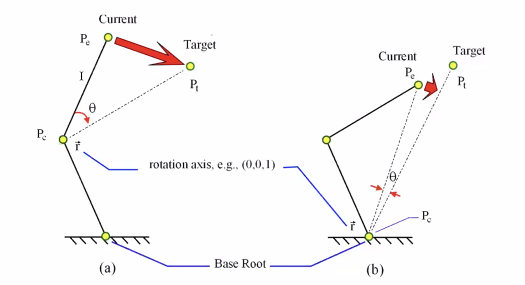
\includegraphics[width=250px]{C:/Users/Alex/Desktop/Notes/Spring 2021/pics/ccd.png}
\end{remark}

\begin{remark}
	Long chains of links tend to wrap up. Can also decide to iterate top to bottom affector or bottom to top. To address this can repeat recursion for every top level: whatever gets recursed more seems to bend more.
\end{remark}

\begin{remark}
	Basic model/fast but some limitations. Fabric better repacement
\end{remark}


\begin{remark}
	Alternative approach is jacobian based inverse kinematics: Introduction to Invers Kinematics with Jacobian Transpose, Pseudoinverse and Damped Leaster Squares
	\begin{verbatim}
		http://math.ucsd.edu/~sbuss/ResearchWeb/ikmethods/iksurvey.pdf
	\end{verbatim}
\end{remark}

\begin{remark}
	We write jacobian as:
	\begin{align*}
		\dot{s} = J(\theta)\dot{\theta}
	\end{align*}

	for speeds on the affectors and their bending angles as we move to a target point. Ie. the change in $s$(position of end affector) against the change in angles.
\end{remark}

\begin{prop}
	\begin{align*}
		\frac{\partial s}{\partial \theta_j} = v_j \times (s - p_j)
	\end{align*}
	where $v_j$ is the axis of rotation for each joint. We take the cross product of line from joint to end affector and rotation axis to get the direction of movement due to that joint(think single arm rotating around line gives tangent to the line)
\end{prop}

\begin{remark}
	To solve $\dot{s} = J\dot{\theta}$ would just want to take inverse but not always possible obviously
\end{remark}

\begin{remark}
	The jacobian transpose always at least does not move away from target: $\langle  J J^T e, e \rangle \geq0$. Often less expensive than pseudoinverse $J^{-1}$ method. 
\end{remark}

\begin{remark}
	For pseudoinverse method we get
	\begin{align*}
		\Delta\theta = J^T(JJ^T)^{-1}e
	\end{align*}
	Note e is $\Delta s$
\end{remark}

\begin{remark}
	Anoter option is damped least squares(really l2 regression). Then
	\begin{align*}
		\Delta \theta = J^T(JJ^T + \lambda^2I)^{-1}e
	\end{align*}

	which we know will be invertible

	Can be solved with line search(grid search) or other techniques
\end{remark}

\begin{remark}
	Example: Want robot hand with 24 degrees of freedom to hit 10 points. So highly underconstrained and thus was resulting in weird, nonnatural solutions. Use Nullspace technique to add some constraint.
	\begin{align*}
		\Delta \theta = J^+e+ (I-J^+J)\phi
	\end{align*}

	want to damp inner joints without affecting result on end affector
\end{remark}

\begin{enumerate}
	\item Resarch progress: 4 hours
	\item Thesis: 5 pages
	\item Clean up lists
\end{enumerate}

\section{2/8}

\subsection{Goals}

\begin{enumerate}
	\item Resarch progress: 4 hours
	\item Thesis: 3 pages
	\item Clean up lists
	\item Text Tessa
\end{enumerate}

\subsection{Complex Analysis}

\begin{theorem}
	If $f$ has primitive then $\int_{\gamma} f(z)dz = F(\omega_2) - F(\omega_1)$
\end{theorem}

\begin{proof}
	Ports from real results by construction.
\end{proof}

\begin{example}
	$\int_{\gamma} dz/z=2\pi i$ where $\gamma$ is unit circle and hence $1/z$ must not have primitive(otherwise would be 0 on closed curve).
\end{example}

\begin{theorem}
	Gauss Lucas
\end{theorem}

\begin{proof}
	Exercise. Very algebraic. Probably write roots as convex combinations. Just compute by taking derivative

	In fact bring out missing roots by taking quotient $P'/P$. Easier to work with these than the complement set of sums and products(often working with quotients easier to access new roots).
\end{proof}

\begin{theorem}
	When $P(z) = \sum a_k a^k$ with real coeffiecients and only real zeroes then coefficients binomial(ultra) log concave.
\end{theorem}

\begin{proof}
	One line proof via gauss-lucas. So derivatives have real roots. Reciprocal poly also has real roots. Then to get the inequality consider $z^{n-k+1}P^{(k-1)}(1/z)$ which has real roots and take $n-k-1$ derivatives resulting in two deg poly. The coefficients of this thing gives desired result by looking at the discriminant.
\end{proof}

\begin{theme}
	This is common technique to show common sequences log-concave
\end{theme}

\begin{example}
	\begin{itemize}
		\item Stirling numbers of first kind
		\item Stirling numbers of second kind
		\item $t_k$ ultra log-concave where $t_k$ number of matchings of size $k$ in arbitrary graph G
	\end{itemize}
\end{example}

\subsection{Technical Animation}

\begin{remark}
	3 techniques for animation: motion capture, procedural, and keyframing.
\end{remark}

\begin{remark}
	CMU Panoptic Studio Dataset: Mocap data
\end{remark}

\begin{remark}
	Motion Capture Data Explained
\end{remark}

\subsection{Random Sign Sums and Hypercube Geometry}

\begin{quest}
Tomaszewski's Conjecture: $P(|X| > 1) \leq 1/2$ for $X = \sum a_i \epsilon_i$?
\end{quest}

\begin{remark}
	Random sign distributions "somewhat" log concave. Ie. log of distribution is log concave
\end{remark}

\begin{theme}
	Random sign sums are like gaussians. 
\end{theme}

\begin{interest}
	To show a probabilistic inequality find an injective map from A to B which is measure preserving. 

	To show $P(|X-a| \leq t) \leq P(|X| \leq t)$ we use reflection of a random walk.
\end{interest}

\subsection{DRL}

\textbf{TAG:} DRL

\subsection{Evolutionary Methods}

\begin{remark}
	Basic reinforcement naive search: randomly choose parameters and see which ones are optimal. Then sample around optimal ones to see if we can do better.
\end{remark}

\begin{quest}
	How do we combat local optimum?
\end{quest}

\begin{ans}
	Restart by initially choosing start parameters uniformly.But certainly not fullproof. In general RL super prone to local optimum.
\end{ans}

\begin{quest}
	Why is our density gaussian and not something else for mutation/parameter updates?
\end{quest}

\begin{ans}
	 I have to assume it's just for ease of computation. Easy to learn and parameterize
\end{ans}

\begin{remark}
	Distributed computing for evolutionary workers has known random seeds
\end{remark}

\subsection{Modeling Evolution}

\textbf{TAG:} ModelingEvolution

\begin{remark}
	Why do we care about a basic model with wrong assumptions? Provides a basis for which we can compare parameters against(for example then varying popluation size and looking at divergence of effects from model).
\end{remark}

\begin{theme}
	Model cost(information cost to store) vs. model explanatory power. Some kind of ratio is the efficiency? Also how do we take into account the computational power necessary to answer questions.

	Applying computational complexity to model theory? Often computational complexity is applied to a single question. But maybe it should be applied to a theory answering a collection of questions? Allows for ammortized analysis of collection of questions.
\end{theme}

\begin{remark}
	How to model? Hard to say except use common sense. very complex. Important to understand what features we want to capture and make sure our model reflects parameters that take this into account.
\end{remark}

\section{2/10}

\subsection{Goals}

\begin{enumerate}
	\item Finish complex homework
	\item Read complex notes	
	\item Research : 3 hors
	\item Thesis : 3 pages
	\item Read Technical Animation Paper
	\itm 1400 Chess
\end{enumerate}

\subsection{Blockers}

\begin{enumerate}
	\item Problem 3 complex
	\item Back problems
\end{enumerate}
	
\subsection{Complex Analysis}

\begin{remark}
	To show mulitiplicative/additive property of exponential show $e^ze^(c-z)$ constant.
\end{remark}

\begin{theorem}
	(Goursout's Theorem): If $\Omega \subseteq \C$ open and $f : \Omega \to \C$ holomorphic with $\Delta \subseteq \Omega$ triangle then 
	\begin{align*}
		\int_{\partial \Delta} f = 0
	\end{align*}
\end{theorem}

\begin{proof}
	Bisect $\Delta$ noting
	\begin{align*}
		\int_{\partial \Delta^{(0)}} f = \int_{\partial \Delta^{(1)}_1} f + ... + \int_{\partial \Delta^{(1)}_4} f
	\end{align*}

	We continue recursively bisecting so that
	\begin{align*}
		|\int_{\partial \Delta^{(k)}} f| \leq 4 |\int_{\partal \Delta^{k+1}} f|
	\end{align*}

	The diameters $d_n \to 0$ and perimeters go to 0 so $\bigcap_{n=1}^{\infty} \Delta^{(n)} = \{z_0\}$(nested compact sets with diameter going to 0).

	We argue
	\begin{align*}
		4^n |\int_{\partial \Delta^{(n)}} f| \to 0
	\end{align*}

	since f is holomorphic. Write $f(z) = f(z_0) + f'(z_0)(z-z_0) + o(z)(z-z_0)$. Clearly $f(z_0)$ and $f'(z_0)(z-z_0)$ have primitives. Thus we are only actually integrating $(z-z_0)o(z)$. Upper bounding $(z-z_0)$ by diameter and $o(z)$ by some $sup_{\Delta^{(n)}} |f(z)|$ we have the bound $p_n d_n \sup$. Recall $p_n = 1/2p_{n-1}$ and $d_n = 1/2 d_{n-1}$ and so we're done.
\end{proof}

\begin{prop}
	Now since we have triangles we can also show for rectangles and by approximation most sets(tesselation). 
\end{prop}

\begin{theorem}
	Let $D \susbeteq \C$ be a disc, $f: D \to \C$ holomorphic then f has a primitive. 
\end{theorem}

\begin{proof}
	Suppose $D$ centered at 0. Write $F(z) = \int_{\gamma_z} f(w)dw$ where $\gamma_z$ is a triangular curve connecting z to 0. 

	Now compute with aim $F(z+h) - F(z) = hf(z)+ho(h) $
	\begin{align*}
		\int_{\gamma_{z+h}} f - \int_{\gamma_z}f = \int_{\gamma{z \to z+h}} f 
	\end{align*}

	by looking at paths and conidering goursout

	Then we conclude by using continuity 
\end{proof}

\begin{remark}
	Notice this argument relies on convexity. The problem is with holes(like the punctured disk).
\end{remark}

\subsection{Technical Animation}

\textbf{TAG:} TechnicalAnimation InverseKinematics

\subsection{Inverse Kinematics}

\begin{remark}
	CCD Illustration:
	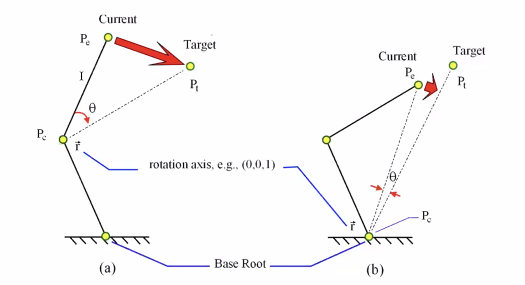
\includegraphics[width=250px]{C:/Users/Alex/Desktop/Notes/Spring 2021/pics/ccd.png}
\end{remark}

\begin{remark}
	Long chains of links tend to wrap up. Can also decide to iterate top to bottom affector or bottom to top. To address this can repeat recursion for every top level: whatever gets recursed more seems to bend more.
\end{remark}

\begin{remark}
	Basic model/fast but some limitations. Fabric better repacement
\end{remark}


\begin{remark}
	Alternative approach is jacobian based inverse kinematics: Introduction to Invers Kinematics with Jacobian Transpose, Pseudoinverse and Damped Leaster Squares
	\begin{verbatim}
		http://math.ucsd.edu/~sbuss/ResearchWeb/ikmethods/iksurvey.pdf
	\end{verbatim}
\end{remark}

\begin{remark}
	We write jacobian as:
	\begin{align*}
		\dot{s} = J(\theta)\dot{\theta}
	\end{align*}

	for speeds on the affectors and their bending angles as we move to a target point. Ie. the change in $s$(position of end affector) against the change in angles.
\end{remark}

\begin{prop}
	\begin{align*}
		\frac{\partial s}{\partial \theta_j} = v_j \times (s - p_j)
	\end{align*}
	where $v_j$ is the axis of rotation for each joint. We take the cross product of line from joint to end affector and rotation axis to get the direction of movement due to that joint(think single arm rotating around line gives tangent to the line)
\end{prop}

\begin{remark}
	To solve $\dot{s} = J\dot{\theta}$ would just want to take inverse but not always possible obviously
\end{remark}

\begin{remark}
	The jacobian transpose always at least does not move away from target: $\langle  J J^T e, e \rangle \geq0$. Often less expensive than pseudoinverse $J^{-1}$ method. 
\end{remark}

\begin{remark}
	For pseudoinverse method we get
	\begin{align*}
		\Delta\theta = J^T(JJ^T)^{-1}e
	\end{align*}
	Note e is $\Delta s$
\end{remark}

\begin{remark}
	Anoter option is damped least squares(really l2 regression). Then
	\begin{align*}
		\Delta \theta = J^T(JJ^T + \lambda^2I)^{-1}e
	\end{align*}

	which we know will be invertible

	Can be solved with line search(grid search) or other techniques
\end{remark}

\begin{remark}
	Example: Want robot hand with 24 degrees of freedom to hit 10 points. So highly underconstrained and thus was resulting in weird, nonnatural solutions. Use Nullspace technique to add some constraint.
	\begin{align*}
		\Delta \theta = J^+e+ (I-J^+J)\phi
	\end{align*}

	want to damp inner joints without affecting result on end affector
\end{remark}

\section{2/11}

\subsection{Goals}

\begin{enumerate}
	\item Finish complex homework
	\item Read complex notes	
	\item Research : 1.5 hours
	\item Thesis : 3 pages
	\item Read Technical Animation Paper
	\item Start technical homework
\end{enumerate}

\subsection{Blockers}

\begin{enumerate}
	\item temp
\end{enumerate}

\subsection{DRL}

\textbf{TAG:} DRL

\begin{remark}
	Natural evolution strategy for distributed model, distributes unique seed to each worker and so do not need to share gradient vectors(only fitness scores)
\end{remark}

\begin{remark}
	Evolutionary methods useful if low number of parameters(100s to 1000s) but has trouble scaling. Need above trick
\end{remark}

\begin{remark}
	Sometimes rewards stochastic, in addition to the actions. Probably because partial information(think gambling).
\end{remark}

\subsection{Multi-Armed bandit}

\begin{remark}
	Winning at slot machines. 
\end{remark}

\begin{remark}
	\begin{align*}
		Q_n = \sum_{R_i}/(n-1)
	\end{align*}

	Is estimate of true q-value(action value)

	Also sometimes problems can be nonstationary ie. action values change. 
\end{remark}

\begin{remark}
	Sample multi-armed strategy: Fix exploration period under which we uniformly sample k-armed bandit and form q values for each action, then take the action which maximizes the reward.
\end{remark}

\begin{remark}
	Other strategies:
	\begin{enumerate}
		\item $\epsilon$ exploration: with prob. $\epsilon$ expore new action
		\item Optimistic: Initialize q values high to incentivize exploration
	\end{enumerate}
\end{remark}

\begin{remark}
	Uncertainty guides exploration: want to explore actions whose expected mean have higher variance
\end{remark}

\begin{remark}
	\begin{align*}
		A_t = argmax_a[Q_t(a) + c\sqrt{log(t)/N_t(a)}]
	\end{align*}
\end{remark}

\subsection{Modeling Evolution}

\begin{remark}
	Mean fitness:
	\begin{align*}
		\theta = ax + by
	\end{align*}
	where
	\begin{align*}
		&\dot{x} = x(a-\theta)\\
		&\dot{y} = y(b-\theta)
	\end{align*}
	and a is fitness of x, b fitness of y
\end{remark}

\begin{remark}
	Modeling heuristic: when product is in differential indicates some kind of mixing of populations
\end{remark}

\begin{quest}
	What determines the "optimal mutation rate". DRL tells us it should be minimal? 
\end{quest}

\begin{ans}
	But if we're too small then the population dies. What would this penalization effect have on DRL setting? What does this mean for rate in evolution?
\end{ans}

\begin{remark}
	Symobls:
	\begin{enumerate}
		\item $V_A = \frac{w_A}{w_a}$ is relative fitness ratio of alleles
		\item $S_d = \frac{w_A - w_a}{w_a}$ coefficient of selection
	\end{enumerate}
\end{remark}

\begin{remark}
This is the haploid picture
	\begin{align*}
		\Delta p = p(t+1) - p(t) = (w_A - w_a)p(t)(1-p(t))/(w_Ap(t) + w_a(1-p(t)))
	\begin{align*}
\end{remark}

\begin{remark}
	Diploid picture: 1 locus, 2 alleles
	\begin{align*}
		\overline{w} = p^2 w_{AA} + 2pq W_{Aa} + q^2 w_{aa}
	\end{align*}
\end{remark}

\section{2/12}

\subsection{Goals}

\begin{enumerate}
	\item Finish complex homework
	\item Read complex notes	
	\item Research : 1.5 hours
	\item Start technical homework
	\item Start DRL
\end{enumerate}

\subsection{Blockers}

\begin{enumerate}
	\item temp
\end{enumerate}

\subsection{Complex Analysis}

\textbf{TAG:} ComplexAnalysis ComplexIntegration

\begin{theorem}
	\textit{Cauchy's Theorem}: If f holomorphic in a disk and $\gamma$ closed curve in disk then $\int_{\gamma} f = 0$. 
\end{theorem}

\begin{remark}
	Cauchy's theorem holds on 
	\begin{itemize}
		\item rectangles
		\item triangles
		\item sectants(triangles with one side smoothed out)
		\item punctured half circle(set removed in neighborhood of 0)
		\item keyhole
	\end{itemize}

	Where we just repeat the same argument as above
\end{remark}

\begin{theme}
	Clever changes of variables are suggested by invariance of the function: for example gaussian rotationally invariant and thus should try polar coordinates
\end{theme}

\begin{remark}
	Rigorously showing fourier transform of gaussian:
	We integrate on some rectangle with width $2R$ centered and with base along $\R$. Call this $\gamma$. We know
	\begin{align*}
		\int_{\gamma} f = 0 = \int_{\gamma_1} f+ \int_{\gamma_2} f + \int_{\gamma_3} f + \int_{\gamma_4} f
	\end{align*}

	with 
	\begin{align*}
		&\int_{\gamma_1} f d = \int_{-R}^R e^{-\pi x^2}dx \to 1\\
		&\int_{\gamma_3} f d = -\int_{-R}^R f(x+iy)dx = \int_{-R}^R e^{-\pi x^2}e^{-2 \pi i xy}e^{\pi y^2} dx
	\end{align*}

	and we see these will agree because the others will go to 0 as $R \to \infty$. 
\end{remark}

\begin{remark}
	This is an example of contour integration: Extracting integral we're interested in by pulling it out as a piece of a contour. In general allows us to compute one integral as another along a different path
\end{remark}

\begin{prop}
	Computing:
	\begin{align*}
		\int_0^{\infty} \frac{1-cos(x)}{x^2}dx = \frac{\pi}{2}
	\end{align*}
	via computing contour for $f(z) = \frac{1-e^{iz}}{z^2}$. We integrate over contour:
	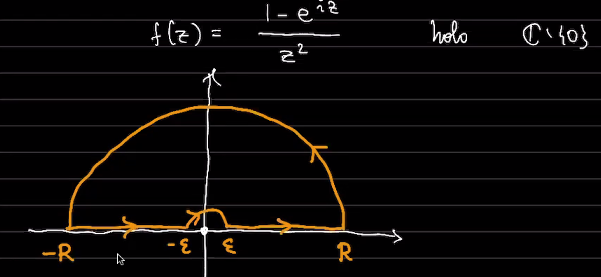
\includegraphics[width=250px]{C:/Users/Alex/Desktop/Notes/Spring 2021/pics/indentedsemicirclecontour.PNG}

	In the limit we'll get what we want. Note integral is 0 to start. So suffices to compute another integral along different path

	\begin{align*}
		\int_{\gamma_{\epsilon}} \frac{1-e^{iz}}{z^2}dz = \int_{\gamma_{\epsilon}} \frac{-iz + g(z)}{z^2}dz = \int_{\gamma_{\epsilon}} \frac{-i}{z}dz = - \pi
	\end{align*}

	where $g(z)$ is remainder of power series which is holomorphic. Value of the integral comes from the singularity
\end{prop}
\begin{theme}
	Note we used linearity of the integral + the powerseries to make integration easier, and recover a holomorphic function(which is often made nonholomorphcic by singularities 1/z)
\end{theme}

\subsection{PDEs and Data}

\textbf{TAG:} OptimalTransport

\begin{theme}
	When trying to solve optimization problems, try to relax problem and solve that, then show is equivalent to original. Primal dual is sometimes example of this
\end{theme}

\begin{reminder}
	Arzela-Ascoli: equicontinuous and uniformly bounded(otherwise could blow up to infinity) functions converge uniformly on compact domains(given some pointwise convergnce). 
\end{reminder}

\begin{remark}
	Optimal trasport maps not unique often(think of point masses on a square).
\end{remark}

\begin{remark}
	Pulling something out of nothing: finding a transport map, playing with necessary conditions:
	\begin{align*}
		y_0 = x_0 - (\nabla h)^{-1}(\nabla \phi(x_0))
	\end{align*}
\end{remark}


\subsection{Complex Analysis}

\begin{theorem}
	\textit{Rigidity}: If $f : \Omega \to \C$ holomorphic, and has $z_n$ which converges in $\Omega$ to $w$, with all $f(z_n) = 0$. Then f = 0
\end{theorem}

\begin{proof}
	First we show f 0 near w. 

	Use power series expansion. AFSOC not 0 near w. Then we have an $a_n \neq 0$. Take minimal one. Compute $f(z) = a_m(z-w)^m(1+g(z))$ where g holomorphic. But as we take a point close enough, we know $f(z_n)$ should be 0 but the product above cannot be. So done in a set

	Let $U = int\{z: f(z) = 0\}$. We know U nonempty. U open, but U also closed because f continuous. Furthermore we can find a neighborhood around z in U(by first part). So it must be U everything since U connected. 
\end{proof}

\begin{prop}
	Uniqueness of analytic continuation. If two holomorphic f,g equal on sequence of points then equal everywhere.
\end{prop}

\begin{proof}
	True by regularity(look at difference). 
\end{proof}

\begin{quest}
	When is there a continuation?
\end{quest}

\begin{ans}
	There should only be a problem at boundary(can think of compact functions going to 0).
\end{ans}

\begin{remark}
	Miracles of holomorphicity: Closedness, regularity, unique extension(rigidity).
\end{remark}

\begin{theorem}
	Morera's Theorem: Converse to cauchy's theorem.

	Suppose $f$ cts on $f : D \to \C$ s.t. for all triangles we have 0 then f holomorphic.
\end{theorem}

\begin{proof}
	From cauchy we know we have $F$ holo on D with $F' = f$.(via this triangle property). Since F holomorphic then f holomorphic. 
\end{proof}

\begin{prop}
	Uniform limits of holo. functions are holo
\end{prop}

\begin{proof}
	If we can show the limit vanishes on triangles then done by Morera. Note we know unif. limits of cts functions are cts. But this is clear just from DCT.
\end{proof}

\begin{remark}
	Recall this does not hold in real case: think weierstrass's theorem(polynomials can uniformly approximate any cts function).
\end{remark}

\begin{theorem}
	Derivative of limit is limit of derivatives of holo. function
\end{theorem}

\begin{proof}
	We go for a bound on the derivative in terms of f: $||F'||_{\infty,\Omega_{\delta}} \leq \frac{1}{\delta}||F||_{\infty,\Omega_{\Omega}}$. This is enough when we look at diferences of the derivatives(take out limit)

	We go by cauchy's formula:
	\begin{align*}
		|F'(z)| = |\frac{1}{2\pi i}\int_{\partial D_{\delta}(z)}\frac{F(w)}{(w-z)^2}dw|
	\end{align*}

	and apply triangle inequality
\end{proof}

\begin{remark}
	True for higher order derivatives. Amazing that knowing holomorphicity gives control of limit of all derivatives. 
\end{remark}

\begin{theme}
	Constructing holomorphic functions: look at series of holomorphic functions(assuming unif. convergence on compact sets)

	Also often useful to define as integrals of holomorphic functions of a parameter.
\end{theme}

\begin{prop}
	Let $F : \Omega \times [0,1] \to \C$. be s.t. 

	i) $z \to F(z,s)$ is holo. for all s

	ii) F cts on $\Omega \times [0,1]$. Then 

	$f(z) = \int_0^1 F(z,s) ds $
\end{prop}

\begin{proof}
	We argue the integral is the uniform limit of the riemanns sums. 

	Write $f_n(z) = \frac{1}{n}\sum^n F(z,k/n)$. Uniform bound comes from continuity: cause we're on a comapct set
\end{proof}

\begin{theorem}
	\textit{Reflection Principle}: Let $\Omega \subseteq \C$ sym. about $\R$. Let $\Omega^+$ be part above real line. Let I be real part. 

	\textit{Symmetry Princple:} Let $f^{+/-}: \Omega^{+/-} \to \mathbb{C}$ holo, both extend cts to I(maybe not holomorphcally). And extensions agree. Then gluing everyting together we get f a holomorphic function. 

	
\end{theorem}

\begin{proof}
	Simply need to check boundary. After showing continuity use morera's theorem(converse to gousard). 

	Hardest case is triangle over interval. Then we simply subdivide and integrate each function along restricted sub-divisions. We use continuous extension by shifting triangles down by $\epsilon$. 
\end{proof}

\begin{remark}
	Real line is irrelevant, can be any curve. Also note holomorphicity is extended by continuity.
\end{remark}

\begin{theorem}
	Schwarz Refletion Principle: Let $f^+: \Omega^+ \to \mathbb{C}$ holo, $f^+$ extends cts to I, $f|_I \in \mathbb{R}$ and reflecting over it.
\end{theorem}

\begin{proof}
	Define $f^-$ and argue using reflection. Set $f^-(z) = \overline{f(\overline{z})}$. Simply need to check holomorphicity(since agreement on real line). 

	To show holo. we use power series. Note bar distributes over multiplication and we're done.
\end{proof}
	
\begin{theorem}
	\textit{Runge's Theorem}: Let $K \subseteq \mathbb{C}$ with f holo. in neighborhood of K. Then f can be approximuated uniformly by rational functions with singularities in $K^C$. 

	If $K^C$ connected then the rational functions can be polynomials. 
\end{theorem}

\begin{proof}
	Use cauchy's formula plus riemann sums. 

	Connectedness(in $K^C$) is used to push away singularities.
\end{proof}

\begin{example}
	$e^{1/z}$ has essential singularity at 0(blows up faster than any rational function at 0). 
\end{example}

\begin{remark}
	We can locally write $f(z) = (z-z_0)^n g(z)$ for a zero $z_0$ of f for g nonvanishing locally.
\end{remark}

\section{2/23}

\subsection{Goals}

\begin{enumerate}
	\item Thesis
	\item Read schnectmann
	\item Technical animation
	\item Start complex
\end{enumerate}

\section{3/1}

\begin{theorem}
	Let f be meromorphic in $\mathbb{C}$ with a rem. sing at $\infty$ or a pole at $\infty$. Then f is rational function.
\end{theorem}

\begin{proof}
	$H = f - f_{\infty} - \sum f_k$. H is entire and bounded and hence constant. Then f must be rational.
\end{proof}

\begin{theme}
	Examine the case at $\infty$ by looking at $f(1/z)$ and the behavior at 0.
\end{theme}

%Often only other people have the baility to distract me from my thoughts: tkocz lecture

\begin{theorem}
	(Argument Principle): $Let f : \Omega \to \mathbb{C}$ meromorphic, $\overline{D}\subseteq \Omega$ a disk. If f has no poles and never vanishes on the boundary then

	\begin{align*}
		\frac{1}{2\pi i} \int_{\partial D} \frac{f'}{f} = \texttt{\#0s - \#poles(in disk)}
	\end{align*}


\end{theorem}

\begin{proof}
	Examine poles and 0s of $f'/f$ and use residue theorem: $\frac{1}{2 \pi i}\int_{\partial D} \frac{f'}{f} = \sum res(f'/f)$
\end{proof}


\section{3/2}

\subsection{Goals}

\subsection{DRL}

\begin{remark}
	Value functions are useful because they capture knowlege of agent regarding how good each state is for goal:
	\begin{verbatim}
		knowledge is represented as a large number of approximate value functions learned in parallel
	\end{verbatim}
\end{remark}

\begin{remark}
	Better policy function: has higher values for all states?
\end{remark}

\begin{remark}
	No need to explore in this search because we will know what happens at every branch. The problem is just to maximize each particular branch
\end{remark}

\section{3/3}

\subsection{Goals}

\subsection{Complex Analysis}

\section{3/4}

\subsection{Goals}

\begin{enumerate}
	\item Finish evolution
	\item Finish complex
	\item Work on thesis
	\item Practice ukulele
\end{enumerate}


\subsection{Complex Analysis}

\begin{theorem}
	Let $f,g$ be holo in $\Omega$ containing closed disk with $|f| > |g|$ on $\partial D$. Then f,f+g have same num zeroes in D.
\end{theorem}

\begin{proof}
	Define $f_t(z) = f(z) + tg(z)$. If $n_t$ is num zeroes in D want it constant. Note $|f_t| \geq |f| - t|g| \geq |f| - |g| > 0$. Ie. dominance is used to remove any zeroes.

	Simply go by argument principle: write
	\begin{align*}
		n_t = \frac{1}{2\pi i}\int_{\partial D} \frac{f_t'(z)}{f_t(z)} dz
	\end{align*}
	by arg principle. Since the LHS is Z valued must be constant(otherwise problems with continuity).
\end{proof}

\begin{theorem}
	Open mapping theorem: Let $f : \Omega \to \mathbb{C}$ be holo, then f is open. 
\end{theorem}

\begin{proof}
	The key is to use Rouche. STS image open since $\Omega$ arbitrary.

	Fix $w_0 \in f(\Omega)$ with $w_0 = f(z_0)$. Set $h(z) = f(z) - w = f(z) - w_0 + w_0 - w = F(z) + G(z)$. We can pick a small enough ball so that $|G| < |F|$ since z fixed. Then we can use Rouche to claim $f(z) - w$ has a zero since $f(z)-w_0$ has a zero. So it must be $D_{\epsilon}(w_0) \subseteq f(\Omega)$. 
\end{proof}

\subsection{DRL}

\begin{remark}
	Generalized policy iteration: interleaving of evaluation and greedification. Must converge. All RL methods version of GPI.
\end{remark}

\begin{remark}
	To find optimal policy in $q^*$, just always take max action. To find optimal policy with $v^*$ 
\end{remark}

\begin{remark}
	Reinforcement learning is efficient alternative to dynamic programming MDP model. We prioritize states to visit instead of treating them all equally.
\end{remark}

\begin{remark}
	Bellman error is difference between bellman equation and $v_*$
\end{remark}

\begin{quest}
	What does it mean to backup a state?
\end{quest}

\begin{remark}
	Backup operators:
		First depends on current policy:
		\begin{align*}
			v_{k+1}(s) = \sum_a \pi(a | s)(r(s,a)+\gamma \sum_{s'}p(s' | s,a)v_k(s'))
		\end{align*}

	while next depends on optimal policy:
	\begin{align*}
		v_{k+1}(s) = max_{a \in A}(r(s,a) + \gamma \sum_{s'\in S}p(s',s,a)v_k(s'))
	\end{align*}
\end{remark}

\begin{remark}
	Monte Carlo methods are used to learn value functions: via estimating with empirical means. No longer have access to full dynamics.
\end{remark}

\begin{quest}
	MC methods seem to work surprisingly well. But in what situations does it not even come close to achieving optimal solution
\end{quest}

\begin{remark}
	Note we do policy improvement on $q$ instead of v since we do not know dynamics and cannot look ahead via actions. So we just have $\pi(s) = argmax_a q(s,a)$
\end{remark}

\subsection{Modeling Evolution}

\section{3/5}

\subsection{Goals}

\begin{enumerate}
	\item Practice singing and ukulele
	\item Finish complex
	\item Research
	\item Work on Thesis
\end{enumerate}

\subsection{Complex Analysis}

\begin{theorem}
	\textit{Max Principle:} Let $f : \Omega \to \mathbb{C}$ be holo, nonconstant. Then f cannot attain a maxim in $\Omega$
\end{theorem}

\begin{proof}
	Suppose $\exists z_0 \in \Omega$ maximal. f open so all values near $f(z)$ are attained. A contradiction.
\end{proof}

\begin{remark}
	Open maps on open sets cannot achive maximua
\end{remark}

\begin{theorem}
	If $f : \Omega \to \mathbb{C}$ holo with $\gamma_0,\gamma_1$ homotopic then $\int_{\gamma_0} f = \int_{\gamma_1} f$
\end{theorem}

\begin{proof}
	   Show integral does not change over small changes in curve and use telescoping trick with approximation trick: bootstrap from circle argument using primitives.

	   very geometric, analytical argument. Not very algebraic. But note these arguments not ameniable to language, hence the length. 
\end{proof}


\begin{theorem}
	Any holomorphic function in a simply conneted comain has a primitive.
\end{theorem}

\begin{proof}
	Let $z_0 \in \Omega$ and write $F(z) = \int_{\gamma} f(w)dw$ where $\gamma$ is joining $z$ to $z_0$. Indepenent of curve via homotopy. 

	Then $f(z+h) - F(z) = \int_{\eta}f(w)dw$ and we get f as the derivative. This also gives us cauchy's theorem
\end{proof}

\begin{remark}
	This definition of simply connected domain not very useful: need one about pathwise connectedness.
\end{remark}

\begin{theorem}
	Let $\Omega$ simply connected with $1 \in \Omega$ and $0 \notin \Omega$. Then in $\Omega$ there is a branch of the logarithm $F(z) = log_{\Omega}(z)$ s.t.
	\begin{enumerate}
		\item F is holomorphic
		\item $e^{F(z)} = z$
		\item $F(r) = log(r)$ when r real and near 1
	\end{enumerate}
\end{theorem}

\begin{proof}
	F is constructed as  primitive of $1/z$. 

	$1/z$ is holomorphic in $\Omega$. Let $log_{\Omega}(z) = F(z) = \int_{\gamma}f(w)dw$ where $\gamma$ connects 1 to z. Clearly F holomorphic.

	We show $ze^{-F(z)} = 1$. Compute
	\begin{align*}
		\frac{d}{dz}[ze^{-F(z)}] = (1-zF'(z))e^{-F(z)} = 0
	\end{align*}

	so done with 2.

	Finally compute for $r \in \R$
	\begin{align*}
		F(r) = \int_1^r \frac{dx}{x} = log(r)
	\end{align*}
\end{proof}

\begin{theorem}
	In the Split plane $\Omega = \mathbb{C}\backslash \{(-\infty,0]\}$ we have the principal branch of log:
	\begin{align*}
		log(z) = log(r) = i\theta
	\end{align*}

	where $z = re^{i\theta}$
\end{theorem}

\begin{proof}
	Integrate first along the real axis then using polar with $1/x$ as primitive.
\end{proof}

\section{3/6}

\begin{enumerate}
	\item Research
	\item Thesis
	\item Finish complex
\end{enumerate}

\section{3/8}

\subsection{Blockers}

\begin{enumerate}
	\item Complex 1.3
	\item Complex 4
\end{enumerate}

\end{document}

